\documentclass[a4paper,12pt]{article}
\usepackage[english]{babel}
\usepackage{bookmark}
\usepackage{amsmath}
\usepackage{amstext} 
\usepackage{amssymb}
\usepackage{color}
\usepackage{graphicx}
\usepackage{listings}
\usepackage{lmodern}
\usepackage{mdframed}
\usepackage{url}
\usepackage{hyperref}
\usepackage{tabularx} 
\usepackage{qtree}
\usepackage{subcaption}
\usepackage{pgfplotstable}
\usepackage{pgfplots}
\usepackage{tikz}

\usepackage[ruled,vlined, linesnumbered]{algorithm2e}
\SetKwRepeat{Do}{do}{while}
\newtheorem{definition}{Definition}[section]
\newcommand{\BlackBox}{\rule{1.5ex}{1.5ex}}

\definecolor{blue}{rgb}{0,0,0.8}
\definecolor{dkgreen}{rgb}{0,0.6,0}
\definecolor{gray}{rgb}{0.5,0.5,0.5}
\definecolor{mauve}{rgb}{0.58,0,0.82}

\lstset
{
   basicstyle=\ttfamily\footnotesize,
   language=C++,
   numbers=right,
   numberstyle=\color{gray},
   showtabs=true,
   breaklines=true,
   breakatwhitespace=true,
   captionpos=bottom,
   keywordstyle=\color{blue},
   commentstyle=\color{dkgreen},
   stringstyle=\color{mauve},
   frame=single
}

\mdfsetup
{
   skipabove=\topskip,
   skipbelow=\topskip,
   leftmargin=2em,
   rightmargin=2em
}
 
\title
{
   
\includegraphics[width=12cm]{up-logo.jpg} \\
   \vspace{2cm}
   \textbf{COS700 Research Report} \\ \vspace{0.5cm}
   \textbf{Genetic Programming for the Automated Design of Cross-Domain Selection Perturbative Hyper-Heuristics } \\ \vspace{0.5cm}
   \textbf{Student number:} u17192968 \\ \vspace{0.5cm}
   \textbf{Supervisor(s)}: \\ Prof. Nelishia Pillay  
}

\author{Rudo Janse van Rensburg}

\date{October 2021}

\begin{document}

\maketitle

\newpage
\linespread{1.241}
\tableofcontents
\newpage
\section*{Abstract}
    \par{
        \noindent 
        Hyper-Heuristics are used as a means of improving the generality of heuristic
        algorithms and have shown great success at solving discrete combinatorial 
        optimisation problems. Creating hyper-heuristics to be applicable across different
        domains, however, proves to be a difficult task given they need to be domain
        agnostic and thus cannot incorporate domain knowledge into their design. Consequently, 
        algorithms have been proposed to automate the process of designing
        these cross-domain hyper-heuristics. This paper propose a novel method of automating 
        the design of selective perturbative Hyper-Heuristics which incorporate Genetic Programming
        such that the classification prowess of Genetic Programming is harnessed.
    }

\section*{Keywords:}
    \par{Automated Design, Cross-Domain, Hyper-Heuristic, Classification, Genetic Programming}

\newpage
\section{Introduction}
    \subsection{Precursor}
        \par{
            \noindent
            The advances of searching algorithms in the realm of Computer Science has
            given rise to informed searches by means of heuristics; which help guide the
            search to mitigate exploring an entire solution space to find an optimal solution. 
            The trend of research has since pushed to generalise algorithms from only
            solving a particular problem in one problem domain, to being able to solve
            problems from multiple domains.\newline 
            \newline 
            To this end, the idea of Hyper-Heuristics has developed, which uses high-level 
            heuristics to traverse a low-level heuristic space rather than a solution space 
            directly, which is more generally applicable to multiple problems from the same 
            problem domain.\newline 
            \newline 
            The potential of Hyper-Heuristics have been further realised in 2011 when the
            Cross-Domain Heuristic Search Challenge (CHeSC 2011) \cite{chesc} prompted competing
            researchers to extend the generalising capacity of their Hyper-Heuristic 
            algorithms to problems from multiple problem domains. Furthermore, this competition gave 
            birth to HyFlex \cite{hyflex2012}, a framework by which researchers could compare
            the performance of their Hyper-Heuristic algorithms, and which will be used in
            this project to evaluate the performance of the proposed solution. 
        }
    \subsection{Objectives}
        \par{ 
            \noindent 
            The paper will propose a novel Selective Pertubative Hyper-Heuristic to pit against
            state-of-art algorithms and determine how well it compares. Thus, in accordance therewith, first 
            objective of the proposed project is to survey and investigate existing
            algorithms that automate the design of Selective Perturbative Hyper-Heuristics
            for solving the discrete combinatorial problems encompassed specifically by the
            CHeSC challenge, in particular algorithms which are represented by classifiers.
            The algorithms investigated here, and their relative performance to the winning
            algorithms of the CHeSC challenge, will be used as a basis for evaluating and
            comparing the performance of the proposed algorithm throughout the developmental 
            and experimental phase of the project.\newline 
            \newline 
            The second objective of the projects encompasses the development and construction of a novel 
            Genetic Programming solution to Automate the Design of Selective Perturbative Hyper-Heuristics, 
            and which specifically represents the tasks as one of a classification nature. The classification 
            capacity of Genetic Programming has been thoroughly demonstrated Espejo Espejo et al. \cite{sgpc}, and it
            is this capacity that the proposed algorithm will attempt to harness.
        }
    \subsection{Layout}
        \par{
            \noindent
            Following this section will be the \nameref{sec:ps}, which will serve to refine the scope and purpose of the paper.
            Thereafter,  \nameref{sec:methodology} will be discussed, encapsulating the research method, experimental setup and 
            will elaborate on implementation details. Following this, will be a \nameref{sec:background} which will include a the 
            literature survey about topics relevant to this research, ensuring the \nameref{sec:relwork} is also presented. This will 
            be followed by a \nameref{sec:discussion}, wherein the algorithm's results will be presented. The \nameref{sec:conclusion}
            tie everything together and summarise the findings of the research.
        }
\section{Problem Statement} \label{sec:ps}
    \par{
        \noindent
        Automated Design of Selective Pertubative Hyper-Heuristics for solving discrete
        combinatorial problems is a relatively well covered domain, in part as a consequence of (CHeSC 2011) 
        and the introduction of HyFlex. Little work has, however, been done on the subject of 
        using Genetic Programming for this purpose, and none of which automate the design in 
        terms of classification; an idea which is has been shown to be successful when using 
        other machine learning techniques.\newline 
        \newline 
        The sole question that this project will attempt to answer is: \newline 
        \newline 
        \textit{How effective can a Genetic Program be used to automate the design of selection perturbative 
        hyper-heuristics when built as a classifier?}\newline 
        \newline 
        This question will be answered by comparing the performance of the proposed genetic program against other
        algorithms that have been applied to the HyFlex problem domains.\newline 
        \newline 
        In accordance with the aforementioned question, the main outcomes of the
        project are as follow:
    }
    \section{Background} \label{sec:background} 
    \subsection{Hyper-Heuristics}
        \subsubsection{Introduction}
            \par{
                \noindent
                Computationally hard search problems often necessitate a means of narrowing
                the scope of the search to avoid traversing an entire search space to find a solution. 
                For this purpose, Heuristics are used. In principal, heuristics serve this
                purpose, however not without a few caveats. For one, the effectiveness of the
                heuristic is reliant on the implementation and expertise of it’s designer, as well
                as domain knowledge of the problem. Furthermore, these heuristics were inherently 
                specialised to a particular problem for which they were designed, and
                could not be applied generally \cite{hyperheuristictas}. To address these, researchers explored
                means of automating the design of heuristics. Whilst this idea of automated
                heuristic design can be traced back to the 1960’s, the term ”Hyper-Heuristic”
                was only coined as recently as the early 2000’s \cite{hyperheuristic2000}. In laymen’s terms,
                hyper-heuristics are heuristics for heuristics. A higher-level hyper-heuristic explores a search space 
                of low-level heuristics which in turn describes the solution space \cite{hhcds}. The low-level 
                heuristics would incorporate the difficulty or quality of a move within the solution space, and 
                the Hyper-heuristic uses these to guide actions of the High-level heuristics.
            }
        \subsubsection{Taxonomy of Hyper-Heuristics}
            \par{
                \noindent 
                Hyper-Heuristics can be classified by 2 primary criteria; the manner in which
                the hyper-heuristic interacts with the heuristic space and the function of the
                low-level heuristics constituting the heuristic space.\newline 
                \newline 
                Conceptually, Hyper-Heuristics interact with low-level heuristics constituting the
                heuristic space in one of two ways; selection or generation.\newline 
                \newline 
                \cite{hhsoa}For a problem domain, either low-level heuristics are nominated to
                create or optimise a solution for the problem - and in this way these low-level
                heuristics are selected - or, new low-level heuristics are created - and this way
                low-level heuristics are generated.
                The difference between the two is in part when and where the low-level heuristic
                is used in the search for a solution and by these attributes can be categorised
                into 2 classes; constructive and perturbative.\newline 
                \newline 
                Typically, constructive heuristics are used to guide the creation of initial solutions
                to a problem which will act as a basis whereupon optimisation techniques
                can build - and in this way is involved in the construction of solutions.
                On the other hand, the function of perturbative heuristics is to improve upon
                existing initial solutions. To explore the Heuristic Space, changes are made to
                an initial solution so as to perturb the solution space, which is explored by the
                Hyper-Heuristic by means of the low-level heuristics.\newline 
                \newline 
                From the 2 aforementioned criteria for classifying Hyper-Heuristics, we end
                up with 4 classes; Selective Constructive, Selective Perturbative, Generative
                Constructive and Generative Perturbative - with Selective Pertubative Hyper-Heuritics being 
                the focus of this research.
            }
        \subsubsection{Selection Perturbative Hyper-Heuristics}
            \par{
                \noindent
                For a particular problem, there are a number of pre-defined low-level 
                perturbative heuristics wh that the Hyper-heuristic will have to choose from. 
                After an initial solution is created, the selective perturbative hyper-heuristic 
                will iteratively apply a selected low-level heuristic to the solution, producing a new
                refined solution. This process of iterative refinement is perpetuated so long as
                there are observable improvements to the solution. The metric by which solutions are 
                evaluated for improvement are problem specific \newline 
                \newline 
                \begin{algorithm}[H]
                    \SetAlgoLined
                    \KwResult{an optimal solution to a particular problem domain.}
                    Create initial solution\;
                    \Do{solutions have improved}{
                        Select a low-level perturbative heuristic to apply\;
                        Apply low-level heuristic to solution\;
                    } 
                    \Return The best solution
                    \caption{How Selective Perturbative Hyper-Heuristics work}
                    \label{alg:sphh}
                \end{algorithm} 
            }
    \newpage
    \subsection{Cross-Domain Hyper-Heuristics}
            \subsubsection{Introduction}
                \par{
                    Cross-Domain Hyper-Heuristics aim to extend the capacity for generalisation,
                    by widening the scope of a hyper-heuristic to multiple domains.\cite{hyperheuristictas}
                }
            \subsubsection{Cross-Domain Heuristics Search Challenge}
                \par{
                    The Cross-Domain Heuristic Search Challenge (CHeSC 2011)\cite{chesc} was a challenge
                    that was held in 2011 which fostered new ideas in the area of research pertaining
                    Cross-Domain Hyper-Heuristics, as well as producing a framework by which
                    to construct these Cross-Domain Hyper-Heuristics; namingly HyFlex\cite{hyflex2012}.\newline 
                    \newline 
                    Given that CHeSC was a competition, it had a set of rules by which competitors
                    had to abide. At the development phase of the competition, competitors were
                    informed of 4 problem domains that their proposed solution would be tested
                    against; namely Maximum Satisfiability, Bin Packing, Permutation Flowshop
                    and Personnel Scheduling. The competition also involved 2 hidden problem domains, 
                    namingly Travelling Salesman and the Vehicle Routing Problem. These
                    hidden problem domains were not divulged to competitors at the development
                    phase of the competition.\newline 
                    \newline 
                    During the testing phase, 3 known domains sampled from the 4 problem domains 
                    as well as both of the hidden domains were used to evaluate the performance 
                    of the competitors’ solutions. It was theorised that the solution that
                    generalised best across domains would have performed better on the unknown
                    domains \cite{hhcds}.
                }
            \subsubsection{HyFlex}
                \par{
                    HyFlex is a Java program which acts as a framework wherein several discrete
                    combinatorial optimisation problems can be solved; namingly Maximum Satisfiability, 
                    One-Dimensional Bin Packing, Permutation Flow Shop, Personnel
                    Scheduling, Travelling Salesman and Vehicle Routing.\newline 
                    \newline 
                    HyFlex includes 4 problem specific categories of low-level perturbative heuristics
                    6for the aforementioned problems, which include Mutational heuristics, Ruin-
                    recreate heuristics, Local search heuristics and Crossover \cite{hyperheuristictas}.
                    Mutational Heuristics function by performing swapping, changing, adding or
                    deletion solution components in accordance with the improvements as determined by an 
                    evaluation function.\newline 
                    \newline 
                    Ruin-recreate Heuristics function by removing parts of a solution, then using
                    problem-specific low-level construction heuristics to build replacements for the
                    removed parts.\newline 
                    \newline 
                    Local search Heuristics function by making minute alterations to randomly se-
                    lected components of a solution and then accepting the changes that are at least
                    as good as the original solution.\newline 
                    \newline 
                    Crossover function by applying crossover operators to a pair of selected solu-
                    tions, producing one offspring which retains aspects of both selected solutions.
                }
    \subsection{Problem Domains}
        \par{
            \noindent  
            \textit{Maximum Satisfiability} -
            This is a problem whereby the satisfiability (whether it can evaluate as True)
            of a given boolean formula needs to be determined by means of assigning any
            boolean value to variables within the formula.\newline 
            \newline 
            \textit{Bin Packing} -
            This is a problem whereby a certain number of items holding different sizes need
            to be placed in a finite number of bins having limited capacity.\newline 
            \newline
            \textit{Permutation Flowshop} - 
            This is a problem whereby a number of jobs need to be scheduled and processed
            on a fixed number of machines with respect to a fixed sequence or order of
            machines.\newline 
            \newline
            \textit{Personnel Scheduling} - 
            This is a problem whereby a Personnel schedule needs to be constructed given
            a plethora of constraints.\newline 
            \newline
            \textit{Travelling Salesman} - 
            This is a problem whereby a Hamiltonian circuit needs to be constructed, where
            cities represent vertexes, and edges are the walks between cities.\newline 
            \newline
            \textit{Vehicle Routing Problem} -
            This a problem whereby the a number of closed routes are scheduled, each taken
            by a vehicle, to perform a sequence of tasks, such that the vehicles start and
            end at a depot.
        }
    \subsection{Genetic Programming}
        \subsubsection{Introduction}
            \par{
                Genetic Programming is a class of Evolutionary Algorithms which, like
                other Evolutionary Algorithms, is a multi-point search which relies on the Darwinian
                principal of Survival of the fittest to iteratively and incrementally evolve
                a population of unfit programs into progressively fitter programs with respect
                to a given problem.\newline 
                \newline
                Genetic Programming is conceptually very similar to Genetic Algorithms, but
                there is one significant difference; Genetic Programs explore a search space
                composed of Programs(i.e. a Program Space), where the objective is to obtain
                optimal behaviours.\newline 
                \newline
                In order to move the search, Genetic Operators are applied to candidates that
                are selected by means of a selection methods which considers the individual’s
                fitness function such that fitter individuals have a greater chance of being selected. 
                In this way, the search is guided towards optimal areas of the Program
                Space.\newline
                \newline 
                \begin{algorithm}[H]
                    \SetAlgoLined
                    \KwResult{a program with optimal behaviour with respect to a particular problem domain.}
                    Create initial population\;
                    \Repeat{a termination criteria is met}{
                        Evaluate the fitnesses of the population\;
                        Obtain parents by means of selection methods\;
                        Apply Genetic Operators to parents to produce offspring\;
                        Incorporate off-spring into the population;
                    }  
                    \Return The best program from the population 
                    \caption{Overview of the Genetic Program algorithm}
                    \label{alg:gp}
                \end{algorithm} 
            }
        
        \subsubsection{Classification}
            \par{
                \noindent
                The process of automating the design of a Hyper-Heuristic will in someway need
                to incorporate the capacity to identify which low-level heuristic to apply given a
                particular solution. With the addition of one layer abstraction, where solutions
                in the solution space are labelled with arbitrary classes, and associate each class
                with predefined low-level heuristic, then the problem becomes one of classification; 
                a function that Genetic Programs have been shown to perform well in
                when compared to a variety of other techniques \cite{sgpc}.\newline 
                \newline 
                There are various representations that can be used to build classifiers with Genetic 
                programs; namingly Arithmetic, Logical, Decision and Production Rule.\newline 
                \newline 
                Arithmetic Trees are trees that are built with Arithmetic operators as their
                function set, and attributes of the data-set as their terminal set.\newline 
                \newline 
                Logical Trees are trees that are built with Logical operators as their function
                set, and attributes of the data-set as their terminal set.\newline 
                \newline 
                Decision Trees are trees where nodes represent attributes of the data-set, and
                edges represent value ranges for the attribute that the node from which they
                stem represents.\newline 
                \newline 
                Production Rule Trees are trees that are built with condition logic, comprising 
                of nodes that represent a logical ”If” operation. These take as arguments a
                condition, an action to take should the condition hold true and finally an action
                to take should the condition not hold. It is this kind of classifier that will be used. 
            }
\section{Related Work}  \label{sec:relwork}
    \par{
        This section will place emphasis on 2 different proposed algorithms 
        which both incorporate classifiers in their algorithm design.\newline 
        \newline 
        In a paper by S. Asta and E. Özcan \cite{astaozcan}, a proposed solution 
        makes use of an Apprenticeship Learning Hyper-Heuristic (ALHH) approach 
        for the Vehicle Routing problem, and compares its performance to that of 
        the winning algorithm of CHeSC 2011, Adaptive Hyper-Heuristic(AdapHH) as well 
        as 2 newer approaches - the P-Hunter algorithm Ip et al. \cite{phunter}   and an algorithm 
        based on Iterated Local Search (AdOr-ILS) proposed by Walker et al. \cite{ILS} . The result of 
        this experiment shows that ALHH outperforming all the competing algorithms and 
        conclusively demonstrates the ALHH’s comparative success in generalizing actions of 
        the expert, even in for unknown problem instances.\newline 
        \newline 
        In another paper Raras et al. \cite{tdnn} , a proposed solutions makes use of a Time Delay Neural
        Network (TDNN) as an apprenticeship learning hyper-heuristic adhering
        to a learning by demonstration approach. The result of the experiment alludes
        empirically to that fact that exposing richer information to the expert has the
        capacity to generate hyper-heuristics with improved generalising capabilities.
        Another paper by Sabar et al. \cite{gehh} proposes a dynamic multi-armed bandit-gene expression programming
        hyper-heuristic for combinatorial optimisation problems(GEP-HH) to automat-
        ically evolve the hyper-heuristic acceptance criteria. The effectiveness of the
        algorithm is demonstrated by evaluating its performance against the top 5 rank-
        ing hyper-heuristics from CHeSC on the problem domains in HyFlex where it
        ranks 4 out of 6; a promising result.\newline 
        \newline 
        Whilst Gene expression programming is a variant of Genetic Programming, the
        approach taken in this paper is removed from the approach of using a classifier to
        select low-level heuristics as observed in the previous 2 papers. This presents a
        gap in research, whereby a Genetic Programming algorithm is used to automate
        the design of Selective Perturbative Hyper-Heuristics for of a classifier.
    }
\section{Methodology} \label{sec:methodology}
    \subsection{Hyper-Parameters}
        \subsubsection*{Maximum Generation} \label{subsubsec:mg}
            \par{
                \noindent
                This parameter represents the termination criteria of the Genetic Program search. When determining a maximum generation it is important 
                not to use too few generations are the search may not have converged and consequently result in underfitting. Using a maximum 
                generation that is to large may result in overfitting.  
            }
        \subsubsection*{Training Percent} \label{subsubsec:kf}
            \par{
                \noindent
                This parameter refers to the portion of the data-set to use when evaluating the quality of invdividuals. 
                A value that is too large will result in the model overfitting and thus hinder generalisation. A value that is too small will result 
                in underfitting.
            }
        \subsubsection*{Main Tree Max Depth} \label{subsubsec:mmd}
            \par{
                \noindent 
                This parameter represents the maximum depth the main program tree (refer to \nameref{subsubsec:representation}) of the Genetic Program may reach. A maximum depth that is to shallow may 
                hinder the learning capacity of the search, whereas a maximum depth that is too deep may result in learning on noise present in the data-set. 
            }
        \subsubsection*{Condition Tree Max Depth} \label{subsubsec:cmd}
            \par{
                \noindent 
                This parameter represents the maximum depth the condition program sub-trees (refer to \nameref{subsubsec:representation}) of the Genetic Program may reach. A maximum depth that is to shallow may 
                hinder the learning capacity of the search, whereas a maximum depth that is too deep may result in learning on noise present in the data-set. 
            }
        \subsubsection*{Population Size} \label{subsubsec:ps}
            \par{
                \noindent
                This parameter represents the number of individual present in each generation (refer to \nameref{subsubsec:controlmodel}) and remains fixed throughout the search. The population size impacts 
                the Genetic Diversity of a population, as more individuals can represent more points in the search space. Thus, a population size that is too small may result in premature convergence on
                local optima. However, a population size that is too large may be unnecessary and result a longer run-times. 
            }
        \subsubsection*{Tournament Size} \label{subsubsec:ts}
            \par{
                \noindent 
                This parameter represents the size of a tournament (refer to \nameref{subsubsec:selection}). A tournament size that is too small may approaches random selection which hinders exploitation.
                A tournament size that is too large results in greater elitism, and thus results in premature convergence. 
            }
        \subsubsection*{Crossover Application Rate} \label{subsubsec:car}
            \par{
                \noindent
                This parameter reprents the percentage of the population that will be produced from Crossover (refer to\nameref{subsubsec:geneticoperators}), and is proportionate to the ease of convegence.
            }
        \subsubsection*{Mutation Application Rate} \label{subsubsec:mar}
            \par{
                \noindent
                This parameter reprents the percentage of the population that will be produced from Mutation (refer to\nameref{subsubsec:geneticoperators}), and is proportionate to the difficulty of convegence.
            }
        \subsubsection*{Hoist Application Rate} \label{subsubsec:har}
            \par{
                \noindent
                This parameter reprents the percentage of the population that will be produced from Hoist (refer to\nameref{subsubsec:geneticoperators}), and is proportionate to the difficulty of convegence.
            }
    \subsection{Genetic Program Algorithm}
        \subsubsection*{Control Model} \label{subsubsec:controlmodel}
            \par{
                \noindent 
                Generational Control Model was used to automate the design of the Selective Perturbative Hyper-Heuristic. Broadly speaking, 
                it entails taking an initial population of candidate individuals representing points in a search space, and iteratively applying 
                genetic operators to a produce new populations, and in this way, traverse the the search space and converging on optimal points therein.  
                \newline     
                \begin{algorithm}[H]
                    \caption{Generational Control Model}
                    \SetAlgoLined
                    \KwResult{A Genetic Program with optimal behaviour.}
                    Create Initial Population\;
                    \Do{Termination Criteria not met}{  \label{alg:gcm}
                        Apply Genetic Operators\;
                    } 
                    \Return An Optimal Program \; 
                   
                    
                \end{algorithm}
                \noindent Each iteration of the loop on line \ref{alg:gcm} is referred to as a Generation, hence the name. 
            }
        \subsubsection*{Initial Population Creation}
            \par{
                \noindent 
                Ramped-Half-and-Half was used to create the initial population (refer to \ref{alg:rampedhalfandhalf}). This is a hybrid approach of the Full method and Grow method so as to produce 
                a genetically diverse initial method, or more technically, represent a greater area of of the program space.\newline 
                \newline 
                \textit{Full} - this will produce a parse tree where each and every branch extends to an imposed maximum depth.\newline  
                \textit{Grow} - this will produce a parse tree where each branch extends at most to an imposed maximum depth. \newline 
                \newline 
                At each depth greater than 2, equal numbers of individuals are created with that imposed depth using Full and Grow. As such, an initial population with 
                parse trees with a wider variety of depths are produced
            }
        \newpage
        \subsubsection*{Representation} \label{subsubsec:representation}
            \par{
                \noindent
                The Genetic Program are production-rule classifiers, whereby the tree is comprised of conditions and and actions to perform 
                when the conditions evaluate true and false respectively.
                    \begin{figure}[!h]
                        \begin{align*}
                            \nonumber 
                            \Tree 
                            [.IF
                                [
                                    .$\leq$
                                    [
                                        .$A_1$
                                    ]
                                    [
                                        .$\times$
                                        [
                                            .$A_2$
                                        ]
                                        [
                                            .$A_3$
                                        ]
                                    ]
                                ]
                                [
                                    .$C_1$
                                ]
                                [
                                    .IF
                                    [
                                        .$\neq$
                                        [
                                            .$A_5$
                                        ]
                                        [
                                            .$A_2$
                                        ]
                                    ]
                                    [
                                        .$C_3$
                                    ]
                                    [
                                        .$C_5$
                                    ]
                                ]
                            ] 
                        \end{align*} 
                        \caption{A simple production rule tree}
                    \end{figure}

                The tree is implemented as a main program tree, where each \textit{IF} has a condition sub-tree associate with it. The output of the condition sub-tree 
                is to be interpreted as a boolean value and this boolean value determines whether the \textit{true} branch \textit{false} gets executed. The condition sub-tree 
                performs relational, arithmetic, bitwise and logical operators on the values of attributes in a data-instances. It is this conditional functionality that allows for learning.\newline 
                \newline 
                It should be noted that the main program tree and the condition sub-trees have their own set of primitives (refer to \ref{def:primitive}).\newline 
                \footnote{
                    \tiny 
                    \begin{definition}\label{def:arity}
                        Arity - The number of arguments a primitive takes.
                    \end{definition} 
                    \begin{definition} \label{def:primitive}
                        Primitive - The nodes of a parse tree.
                    \end{definition} 
                    \begin{definition}\label{def:terminal}
                        Terminal - A primitive that takes no arguments,i.e has an arity of 0.
                    \end{definition} 
                    \begin{definition} \label{def:function}
                        Function - A primitive that takes arguments,i.e has an arity of at least 1.
                    \end{definition} 
                }
                \newpage
                \noindent \textbf{Main Program Tree} \newline 
                The sole function(refer to \ref{def:function}) of the main program tree is the \textit{If} function. It takes in 3 arguments; a condition body to evaluate, a body of code 
                to execute if the condition evaluates true and a body of code to execute if the condition evaluates false. The sole terminal(refer to \ref{def:terminal}) is the class terminal, which represents
                a class of the classifier. \newline 
                \newline 
                \noindent \textbf{Condition Sub-Tree} \newline 
                The sole terminal of the condition sub-tree is the attribute terminal, which represents the value of an attribute in the instance being classified. 
                The function set is comprised of 4 categories of operations - relational, arithmetic, bitwise and logical - and each take 2 arguments. Relational functions include 
                $>,<,\leq,\geq,\neq$. Arithmetic functions include $+,-,\div,\times$. Bitwise functions include $\|, \&$. Logical functions include $OR, AND$.
                \begin{figure}[h!]
                    \begin{minipage}[c]{0.5\textwidth}
                        \centering
                        \begin{tabular}{|c|c|c|}
                            \hline
                            \textbf{Function} & \textbf{Arity} & \textbf{Tree}\\
                            \hline
                            IF & 3 & Main  \\
                            \hline 
                            $>$ & 2 & Condition \\
                            \hline
                            $<$ & 2 & Condition \\
                            \hline
                            $\geq$ & 2 & Condition \\
                            \hline
                            $\leq$ & 2 & Condition \\
                            \hline
                            $+$ & 2 & Condition \\
                            \hline
                            $-$ & 2 & Condition \\
                            \hline
                            $\div$ & 2 & Condition \\
                            \hline
                            $\times$ & 2 & Condition \\
                            \hline
                            $\|$ & 2 & Condition \\
                            \hline
                            $\&$ & 2 & Condition \\
                            \hline
                            $\oplus$ & 2 & Condition \\
                            \hline
                            $\text{OR}$ & 2 & Condition \\
                            \hline
                            $\text{AND}$ & 2 & Condition \\
                            \hline
                        \end{tabular}
                        \subcaption{Functions}
                    \end{minipage}
                    \begin{minipage}[c]{0.5\textwidth}
                        \centering
                        \begin{tabular}{|c|c|c|}
                            \hline
                            \textbf{Terminal} & \textbf{Arity} & \textbf{Tree}\\
                            \hline
                            Class & 0 & Main \\
                            \hline
                            Attribute & 0 & Condition  \\
                            \hline  
                        \end{tabular}
                        \subcaption{Terminals}
                    \end{minipage}
                    \caption{Summary of Primitives}
                \end{figure} 
            }
        \newpage
        \subsubsection*{Genetic Operators}\label{subsubsec:geneticoperators}
            \par{
                \noindent \textbf{Crossover} - Crossover is a local-search operator that drives convegence by exploiting what has been explored by the search space. It accomplishes this 
                by selecting (refer to \nameref{subsubsec:selection}) a pair of candidate parents from the population, uniformly randomly selecting crossover-points on each parent, then swapping the sub-trees rooted 
                at those points on each tree. In this wasy, genetic material is combined from both parents. To ensure that trees maintain there validity strong-typing is 
                enforced, whereby only nodes in the main tree can be crossed over with one another, and only nodes in the condition sub-trees can be crossoved over with
                one another.\newline 
                \newline 
                \textbf{Mutation} - Mutation is a global-search operator that drives divergence by exploring areas of the search space. It does this by selecting a sole candidate
                parent from the population, uniformly randomly selecting a mutation-point, then recreating the sub-tree rooted at that point. In this way, new genetic material is 
                introduced and thereby enhancing genetic diversity of the population.\newline 
                \newline 
                \textbf{Hoist} - Hoist is an operator with both explorative and exploitative qualities. It accomplishes this by selecting a parent from the population, 
                uniformly randomly selecting a hoist-point, then making that point the root of the off-spring. In this way, it exploits the genetics of its parent, while exploring 
                the neighbourhood thereof. 
            }
        \subsubsection*{Selection Method} \label{subsubsec:selection}
            \par{
                A selection method is a means by which to nominated candidates to apply genetic operators to - producing offspring. The selection method is a function of the the fitness (refer to \nameref{subsubsec:objectivefunction}),
                such that fitter individuals have a greater chance of being nominated. Note that poorer candidates can be nominated, however unlikely, so as to mitigate \textit{Elitism}, which ultimately
                causes premature convergence by impeding genetic diversity.\newline 
                \newline 
                For the purpose of selection, \textbf{Tournament Selection} is used in this experiment. A number of individuals (refer to \nameref{subsubsec:ts}) are uniformly randomly chosen to enter a 
                tournament. The individual with the best fitness (largest in the case of a maximisation, smallest in the case of minimisation) is the winner of the tournament, and it is used as the candidate parent. 
            }
        \newpage
        \subsubsection*{Objective Function} \label{subsubsec:objectivefunction}
            \par{
                \noindent The objective function is used as the "fitness" of the individual, and it is this that the \nameref{subsubsec:selection} uses to nominate candidates 
                for partipation in \nameref{subsubsec:geneticoperators}. \newline 
                \newline 
                Given that the Genetic Program represent a classifier, it's fitness should assess it's classifying ability. For this purpose, the classifier's \textbf{F1 Score} \cite{f1score} is used.
                \begin{figure}[h!]
                    \begin{minipage}[c]{0.5\textwidth}
                        \begin{align*} 
                            \nonumber F_{1} =  \frac{tp}{tp + \frac{1}{2}(fp + fn)}
                        \end{align*}
                    \end{minipage}
                    \begin{minipage}[c]{0.5\textwidth}
                        \begin{align*} 
                            \nonumber tp &- \text{true positives} \\
                            \nonumber fp &- \text{false positives} \\
                            \nonumber fn &- \text{false negatives} \\
                        \end{align*}
                    \end{minipage}
                    \caption{The $F_1$ score}
                \end{figure} 
            }
    \subsection{Data-set}
        \par{
            \noindent The data-set used to train the classifiers is quintessential in allowing the classifiers to make inferrences and learn about the 
            Heuristic space, and by extension, how effective the Hyper-Heuristic will be.  
        }
        \subsubsection*{Data-Engineering}
            \par{
                The data-set is not wholely original, as it was derived from the data-set used by Raras et al. \cite{tdnn}, whereby a memory of the last 8 changes in objective 
                function where used to select one of 12 low-level heuristics as specified within HyFlex and described in a paper by Walker et al. \cite{ILS}. However, their proposed algorithm (and the data-set) where specific to the HyFlex Open Vehicle Routing 
                problem. For the purpose of producing a cross-domain Hyper-Heuristic, the data-set required to be adjusted.\newline 
                \newline 
                One glaring problem with using the data-set used by Raras et al. \cite{tdnn} is that not all Problem Domains in the CHeSC 2011 competition have the same number
                of low-level heuristics, nor are the low-level heuristics necessarily the same. However, each and every problem domain has the same number of 
                low-level heuristic categories. Thus, in order to make the data-set more generally applicable (to different problem domains), the low-level heuristics need to be 
                mapped to their respective categories. 
                \newline
                \begin{table}[ht]
                    \centering
                    %\begin{center}
                        \small 
                        \begin{tabular}{ | c | c | } 
                            \hline
                            \textbf{Parameter} & \textbf{Category} \\
                            \hline  
                            Two-Opt & Mutational \\
                            \hline 
                            Or-Opt & Mutational \\
                            \hline 
                            Shift & Mutational \\
                            \hline 
                            Interchange & Mutational \\
                            \hline 
                            Time-based radial ruin & Ruin and Recreate \\
                            \hline 
                            Location-based radial ruin & Ruin and Recreate \\
                            \hline 
                            Shift & Local Search \\
                            \hline 
                            Interchange & Local Search\\
                            \hline 
                            Two-opt & Local Search \\
                            \hline 
                            GENI & Local Search \\
                            \hline
                            Combine & Crossover \\
                            \hline
                            Longest Combine & Crossover \\
                            \hline
                        \end{tabular}
                        \caption{The 8 low-level heuristics and their Categories.} 
                   % \end{center}
                \end{table}
                To further enhance the data-set, a memory buffer of the last 8 low-level heuristic selected are engineered, in line with the memory buffer of 
                the last 8 deltas (change in objective function). \newline 
                \newline 
                Finally, we have a dataset in which a state $s_i$ is defined in equation \ref{eq:state}
                \begin{equation} \label{eq:state}
                     s_{i} = \{ d_{i}, h_{i}, d_{i-1},h_{i-1},...,d_{i-n},h_{i-n} \} 
                \end{equation} 
                Where $d_i$ is the change in the objective function from iteration $i-1$ to $i$ and $h_i$ is the heuristic applied to $s_{i-1}$ to get to state $s_i$.
            }
    \newpage
    \subsection{Algorithm}  
        \par{
            \noindent The algorithm has 2 phases; the training phase and the problem-solving phase.\newline 
            \newline 
            \textbf{Training} - Part of the first phase involves  creating an initial population by means of the 
            Ramped-Half-and-Half method, which Algorithm \ref{alg:rampedhalfandhalf} describes.
            \begin{algorithm}
                \caption{Ramped Half-and-Half Method} 
                \label{alg:rampedhalfandhalf}
                \SetAlgoLined
                \SetKwInOut{Input}{inputs}
                \SetKwInOut{Output}{output}
                %Function Definition%
                \SetKwProg{CreateInitialPopulation}{CreateInitialPopulation}{}{}
                \CreateInitialPopulation{$(P,D_{max})$}{
                    \Input{Population size $P$; an \texttt{Max Depth} $D_{max}$}
                    \Output{An \texttt{Population} denoted by $G$}
                    %Function Body% 
                    $G \gets \emptyset$ \; 
                    \ForEach 
                    {
                        %ForEach Condition%
                        $d \in \{x \| x \in \mathbb{Z} \wedge 2 \leq x \leq D_{max} \}$
                    }
                    {
                        $i \gets 0$ \;
                        %ForEach Body%
                        \For
                        {
                            %For Condition%
                            $i <\frac{1}{2}\frac{P}{D_{max} - 2}$
                        }
                        {
                            %For Body%
                            $G \gets G \cup  Grow(d)$ \;
                            $G \gets G \cup  Full(d)$ \;
                            $i \gets i + 2 $\;
                        }
                    
                    } 
                    %Return value%
                    \KwRet{$G$}\;
                 
                } 
            \end{algorithm}
            \noindent Thereafter, the initial population will be evolved until a predefined maximum generation, which effectively automates the design of
            our Selection Hyper-Heuristic. 
            
        }
    \newpage
    \subsection{Experimental Setup}
        \subsubsection*{Training}
            \par{
                \begin{figure}[h!]
                    \begin{center}
                        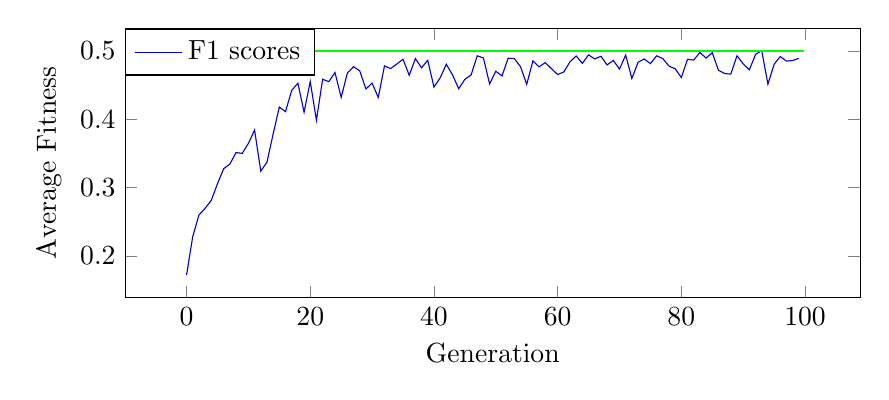
\begin{tikzpicture}
                            \centering
                            \begin{axis}[
                                xlabel=Generation,
                                ylabel=Average Fitness,
                                width=0.9\textwidth,height=5cm,
                                legend style={at={(0.0,.91)},anchor=west}
                            ]% Add values and attributes for the first plot 
                                \addplot[color=blue,mark=.] coordinates {
                                    (0,0.1720092351746414 )
                                    (1,0.22827411458135435 )
                                    (2,0.2598164508107516 )
                                    (3,0.2695748560021816 )
                                    (4,0.2813380513609234 )
                                    (5,0.30563668282185963 )
                                    (6,0.3275982788561947 )
                                    (7,0.33439596636803476 )
                                    (8,0.3511874210524675 )
                                    (9,0.3501013453703306 )
                                    (10,0.3646729305581925 )
                                    (11,0.38412688457908883 )
                                    (12,0.3240496684890505 )
                                    (13,0.3371717651660749 )
                                    (14,0.3784134202171267 )
                                    (15,0.4178680234432069 )
                                    (16,0.4110946823320159 )
                                    (17,0.44229304922064017 )
                                    (18,0.4527064143366971 )
                                    (19,0.410346486447574 )
                                    (20,0.45526793137752586 )
                                    (21,0.3984897698564815 )
                                    (22,0.45859274042686204 )
                                    (23,0.4550616981965662 )
                                    (24,0.4684706097241164 )
                                    (25,0.43199697096366557 )
                                    (26,0.4675557471530718 )
                                    (27,0.4769742830535652 )
                                    (28,0.4708552489100829 )
                                    (29,0.4443600245599349 )
                                    (30,0.4528749552127181 )
                                    (31,0.431982295129391 )
                                    (32,0.47809286463876055 )
                                    (33,0.47424643321872717 )
                                    (34,0.4808699812420769 )
                                    (35,0.48791072881621295 )
                                    (36,0.4644563660055484 )
                                    (37,0.48875317042938127 )
                                    (38,0.4754087950501023 )
                                    (39,0.4863014985104761 )
                                    (40,0.44721391675442995 )
                                    (41,0.4605080061387104 )
                                    (42,0.4805316279651172 )
                                    (43,0.46503345891961617 )
                                    (44,0.44471870033420474 )
                                    (45,0.4585329287540254 )
                                    (46,0.4647678674148425 )
                                    (47,0.4929385786376247 )
                                    (48,0.48980777548675863 )
                                    (49,0.45179775018853 )
                                    (50,0.47034410061340026 )
                                    (51,0.4634821628146253 )
                                    (52,0.4893602666417894 )
                                    (53,0.48879856654320764 )
                                    (54,0.4770386129987109 )
                                    (55,0.4510476389457079 )
                                    (56,0.4854322077679282 )
                                    (57,0.47674788486645864 )
                                    (58,0.48294279212821567 )
                                    (59,0.4740795420207156 )
                                    (60,0.46546546315141285 )
                                    (61,0.4692071530383252 )
                                    (62,0.48420028639710283 )
                                    (63,0.49260994731864777 )
                                    (64,0.4819016411804831 )
                                    (65,0.49432755563455083 )
                                    (66,0.48831457920891264 )
                                    (67,0.49220082474127874 )
                                    (68,0.47952326320035765 )
                                    (69,0.4862466024884558 )
                                    (70,0.47345486459775393 )
                                    (71,0.4938709459837964 )
                                    (72,0.45973910721005834 )
                                    (73,0.4833415778279418 )
                                    (74,0.48830749224691905 )
                                    (75,0.48139967750790535 )
                                    (76,0.4928672476242067 )
                                    (77,0.48894953753675485 )
                                    (78,0.477832584576695 )
                                    (79,0.47393054525311207 )
                                    (80,0.4611256647471626 )
                                    (81,0.4877673688421303 )
                                    (82,0.48668456474301475 )
                                    (83,0.4978151894055181 )
                                    (84,0.489637828636316 )
                                    (85,0.497389539557108 )
                                    (86,0.47179599282805157 )
                                    (87,0.46698047035273477 )
                                    (88,0.4660732331619189 )
                                    (89,0.49297040452169755 )
                                    (90,0.4811752251850691 )
                                    (91,0.4724037548034369 )
                                    (92,0.4949612856678532 )
                                    (93,0.5004553340718693 )
                                    (94,0.45136577553634605 )
                                    (95,0.480487351538623 )
                                    (96,0.4918244219391049 )
                                    (97,0.48511625417198345 )
                                    (98,0.48597528362491393 )
                                    (99,0.4892341187324779)
                                };
                                \addplot[color=green,mark=-] coordinates {
                                    (0,0.5) 
                                    (99,0.5)
                                };
                                \legend{F1 scores}
                            \end{axis}
                        \end{tikzpicture}
                    \end{center}
                    \caption{Graph showing the average score of each generation}
                \end{figure} 
                \noindent From the graph, it is clear that the algorithm converged as after about generation 40 the graph plateaus. 
                
            } 
        \subsubsection*{Parameter Values}
            \par{
                The parameter values were determined empirically.
                \begin{table}[h!]
                    \centering
                    %\begin{center}
                        \small 
                        \begin{tabular}{ | l | c | }

                            \hline
                            \textbf{Parameter} & \textbf{Value} \\
                            \hline  
                            \nameref{subsubsec:mg} & 100 \\ 
                            \nameref{subsubsec:kf} & 0.7 \\ 
                            \nameref{subsubsec:mmd} & 10 \\ 
                            \nameref{subsubsec:cmd} & 5 \\ 
                            \nameref{subsubsec:ps} & 2000 \\ 
                            \nameref{subsubsec:ts} & 4 \\ 
                            \nameref{subsubsec:car} & 0.5 \\ 
                            \nameref{subsubsec:mar} & 0.475 \\ 
                            \nameref{subsubsec:har} & 0.5 \\
                            \hline 
                        \end{tabular}
                        \caption{Parameter values used in the experiment.} 
                % \end{center}
                \end{table} 
            }
       

\section{Discussion} \label{sec:discussion}
    \par{

    }
\section{Conclusion} \label{sec:conclusion}
    \par{

    }
\newpage
% \bibliographystyle{ieeetr}
\bibliographystyle{alpha}
\bibliography{myBibFile} %change the name here to the name of your .bib file

\end{document}